\chapter{Design}
\label{cha:design}

Given our purpose for the game, it is important that the game is accessible to the user.
This means, that the user intuitively knows have the game is supposed to work, and how success within the game can be achieved.
The challenge will then be to create a game, which manages to educate, while maintaining engaging gameplay for the user.
Many ideas to do this is described in the analysis part of this report.
The following sections will describe the initial design ideas, and how a solution that achieves this could look in the early stages of the design phase.

\section{Game Environment}
\label{sec:game_environment}

Given our purpose for the game, it is important that the game seems immediately accessible to the user. This means, that the user intuitively knows have the game is supposed to work, and how success within the game can be achieved.
The challenge will then be to create a game, which manages to educate, while maintaining excitement for the user.
The following sub-sections will describe the initial design ideas, and how a solution that achieves this could look in the early stages of the design phase.

\subsection{Gameplay}

The game is intended to be a competitive \textit{'who-has-the-best-algorithm-to-solve-a-problem-on-a playing-field'} type of game.
The player will initially be in charge of a single simple biological cell with the ability to consume food on the playing field, evolve, and grow larger. The game is finished, when one player's cell has grown larger than the opponent's cell, and opponent's cell has been consumed.
There will be multiple actions available to each player's cells, for example;
\begin{itemize}
	\item Move in a given direction.
	\item Consume food.
	\item Try to consume an opponent cell
	\item Split their cell - evenly partitioning their cell and creating a copy.
\end{itemize}
%they may chose to split-up their cell - evenly partitioning their cell and creating a copy, allowing the player to control more cells on the playing field, they could move it in a given direction, they could try to attack the other player, or perhaps they go scavenging for food.
The player programs their single cell before a game begins in an easy-to-use drag-and-drop interface.

\subsection{Programming the Cell}

Programming the cell should be inviting to the user, and not be the cause of frustration due to the occurrence of peculiar programming-oriented errors, they will be tasked to dealing with.
For this reason, it is important that the interface provides the user with feedback which gives a clear understanding of when the user has combined a string of legal or illegal programming constructs.
In general terms, it is important that the user cannot make too many construction mistakes.
Otherwise the game could become a game about debugging, when it should be a game about creating the most optimized and best algorithm/cell.

\subsection{Playing Field}

The playing field is the map on which the cells compete.
It is a 2D environment, which is split up into tiles making the playing field a grid.
Splitting the map into tiles will make it easier to solve problems such as, is a given cell within attacking range of an opponent cell, or is a given cell standing on food or some other item of interest.
Doing this will limit the freedom each user has in terms of moves and gameplay, however, since cells cannot move freely in the 2D environment (a complete 360 degrees) or make exactly the decision they may want to make. 
So as a compromise to this limitation, the group decided to use hexagonal tiles, which is also used in the blockbuster game title Civilization 5.\todo{Find eventuelt den talk Sid Meier afholder omkring Hexagons i CIV 5 og hvorfor det er superr duperr}
\section{Designing the Behavior of Cells}
\label{sec:designingBehaviorCells}

The behavior of each cell is defined by the player, since it is his/her job to program the behavior \todo{ref to designing of programming interface selection}.
However, this section will focus on the standard actions that all cells can perform and how they work.
We will also discuss other possible implementations of attributes for cells, that might include strength, speed, and vision.

\subsection{Standard Actions}

%The player will initially be in charge of a single organic cell with the ability to consume red blood cells or enemy infecting cells.
The player will initially be in charge of a single organic cell with the ability to consume stars\todo{We use stars instead of red blood cells} or enemy infecting cells.
This is done automatically if a cell moves to a tile where either a star or enemy is placed.
%The red blood cells contain oxygen, which works as a nutrient to the cell, and consuming enemy cells will also work as a nutrient, but only if the enemy cell is smaller than the players cell.
The stars contain energy, which works as a nutrient to the cell, and consuming enemy cells will also work as a nutrient, but only if the energy of the enemy cell is smaller than the energy of the players cell.
%These red blood cells are placed on the playing field, see \autoref{sec:designing_playing_field}, and consuming them will allow the initial cell to grow larger/gain health, and evolve.
These stars are placed on the playing field, see \autoref{sec:designing_playing_field}, and consuming them will allow the initial cell to grow larger/gain energy, and evolve.
Evolution can be implemented by either allowing players to modify their cells while the game is played by editing their code or by splitting the cell up into two cells.
The game is finished, when one side does not have any more cells left on the board.\newline

When the cells are on the board, they use energy for every turn, so a cell with an energy level of $100$ would have an energy level of $99$ after one turn on the board regardless of the action that cell has done. The same is true for the stars, which will also decrease in energy level over time.\todo{I can not explain why this is done, but maybe someone else can}\newline

Before the cells are released onto the playing field, the player will program the initial cell in a block structure similar to that of 'Carnage Heart' and 'Kodu Game Lab'.
In this block structure, the player will have multiple actions to implement, that is available to the initial cell and all future evolutions of that cell.
These standard actions include:\newline

\verb|Move(x:steps, y:direction)| is an action that moves the cell $x$ steps in $y$ direction.
Steps can only be positive integers, and might be limited by an ability or the energy of the cells that performs the move action.
Since the playing field consists of multiple hexagonal tiles, each cell can move in six directions.
Direction is an enum type, that can have the values (TopRight, TopLeft, BottomRight, BottomLeft, Left or Right).\todo{check later}\newline

\verb|Look(x:lookingFor, y:direction, z:trigger)|\newline 

%\verb|Consume()| is a function that, if the cell is standing on a tile containing a red blood cell or a smaller enemy cell, will make the cell consume the cell and either use the oxygen in the red blood cell or the energy in the opponent cell to grow.
%The amount of oxygen in each red blood may vary and increases over time.\newline

%\verb|Attack(y:direction)| attacks the tile in the y direction. If this tile contain an enemy cell with less health than the attacking cell, then the attacking cell will consume the enemy cells health and move to that the tile, that the enemy was standing on. If the enemy has greater health than the attacking cell, the attacking cell will be consumed completely by the enemy.\newline

\verb|Split(a:energy, y:direction)| splits the cell into two cells in the $y$ direction, where the new cell get $a$ amount of energy from the splitting cell and is place on the tile in the $y$ direction from the splitting cell.
$a$ is restricted by the energy of the splitting cell, since all cells must have a minimum energy level of $1$.
If a cell is on the edge of the playing field, it is possible to split so the new cell is placed outside the playing field, which will result in the death of the newly created cell.

\section{Designing the Playing Field}
\label{sec:designing_playing_field}
As stated in the requirements section, the game will be displayed as a 2D environment instead of 3D, since the focus of this project is not on the graphical presentation of the game, but on the combination of engagin gameplay and education. However, there are still different approaches when designing the playing field. This section will focus on these approaches and argue why some solutions have been chosen over others. We will use our own game, where the player programs a cell to move around the environment to eliminate enemy cells a an example.

\subsection{Free Environment vs. Tile-styled}

When approaching the design of a 2D environment, it might be possible to design the layout as being free or limited.
In a free environment, the cell would be able to move in all 360$^{\circ}$.
This approach is seen in the game \textit{Osmos}, that is similar to our game without the programming aspect.
The player can move a cell freely in the 2D environment to eat smaller cell and each level has a specific objective.
However, the free environment approach would possibly increase the difficulty of programming the cell in contrast to a tile-styled approach to design.
Note, that by tiles we do not mean traditional tiles, such as those used in \textit{Mahjong} and \textit{Domino}, but rather games were the playing field is made by the players at the beginning of game by laying tiles with different properties.
The tile-style is known from board games, such as \textit{The Settlers of Catan} and \textit{Hive}, where both board games use hexagonal tiles.
However, tiles may not be restricted to being hexagonal, but we will discuss this later in this section.\\

Using tiles would limit the available movements of each cell into $x$ number of directions, where $x$ denotes the amount of sides on a single tile. This limiting factor would make it easier for the player to program each cell, because for example 6 movement options are much less than 360. The question is then whether the tile-styled approach would limit the player too much, making the game less engaging and too easy. However, the same question can be applied to the free environment approach.\\

We have chosen to design the playing field as a tile-styled board game, since we do not think that the limitation of tiles makes the programming of the cells too easy. It might even increase the user base, by allowing less experienced player to program cells that have a chance to defeat more experienced players. This also effects the more experienced players, since, if multiplayer is implemented, the experienced players will then face more difficult cells. We judge, that the sense of achievement when having defeated a difficult opponent is greater than when the opponent is weak and easy to defeat.\\

However, as mentioned easier, tiles can have $x$ number of sides. The next subsection will focus on how to design the tiles in terms of number of sides on each tile and whether tiles should include different properties.

\subsection{Designing the Tiles - Polygons}

Polygons are closed 2 dimensional object that have more than 2 sides. The smallest polygon in term of sides is therefore the triangle. \textit{Bizingo} is a board game that use triangle tiles, but we have not been able to find other games. It is far more common to see games that use either square or hexagonal tiles. These approach therefore both have the appeal of being more recognizable to the user. We will mainly discuss the pros and cons with square and hexagonal tiles.\\

\todo{Discuss why hex are better than square tiles}




\section{Architecture}
\label{sec:architecture}

This section will focus on the chosen architecture for our game.
There exist different architecture, but we have look at the client-server model, peer-to-peer model and model view controller as possible candidates.
We first describe our chosen architecture and then present the alternatives.

\subsection{Client-Server Model}
Our application will make use of the Client-Server model, a model that consists of two parts, a client and a server.
The basic structure of the client-server model can be seen in \autoref{fig:client-server}.

\begin{figure}[ht]
  \centering
    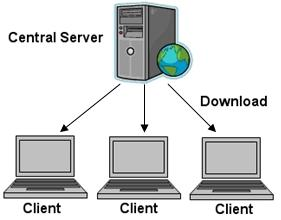
\includegraphics[width=0.5\textwidth]{img/client_server.jpg}
  \caption{Client-Server Technology \citep{ClientServer}}
  \label{fig:client-server}
\end{figure}

The client runs on the users PC, and is responsible for rendering the graphics and gameplay in the users browser.
This is done locally, without the need to connect to a server.
The client will connect to the server over the internet to receive information such as leaderboard statistics.
If multiplayer is implemented, multiple clients could be able to play against one another by connecting to a central server.
The server would then match the two or more players against each other in the same game and keep track of their individual progress.
Depending on how this is implemented, the server could also be running the clients programs.
This could be a relevant implementation for a multiple of reasons.
One reason would be to prevent cheating.
If the server executes the programs, situations where the client is modified to increase the number of points given or the time taken to solve a problem could be avoided.\todo{Other reasons?}

\subsection{Alternative Models}
\subsubsection{Peer-to-Peer}
An alternative to the Client-Server model is the Peer-to-Peer model.
The Peer-to-Peer model is like the Client-Server model without the server.
Instead all the clients connect to each other in a decentralized system, as seen in \autoref{fig:p2p}.

\begin{figure}[ht]
  \centering
    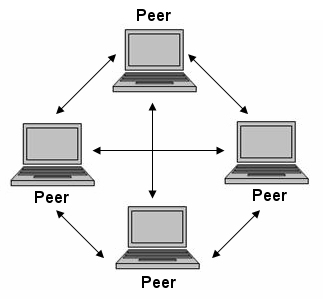
\includegraphics[width=0.4\textwidth]{img/p2p.jpg}
  \caption{Peer-to-Peer Technology \citep{PeerToPeer}}
  \label{fig:p2p}
\end{figure}

One of the positive aspects of this model is, that it drastically reduces the cost that a Client-Server based system has to keep servers running by avoiding the server completely.
However, the Peer-to-Peer model also has some negative features.
One of these features is that because most of the peers in a Peer-to-peer system are PC's, they may not always be available, and thus if no or few people are playing the game, it becomes difficult to play at all.
Another negative feature is that the prevention of cheating becomes more difficult, since it is possible to have player clients run each others programs, but modified clients can still take over the system and corrupt the results.\newline

\subsubsection{Model-View-Controller}
The Model-View-Controller design pattern separates the representation of information from a user's interaction with it.
MVC is often used in web applications and consists of three separate parts, model, view, and controller.
Due to the separation of data and user input, it is possible to have multiple different views for the same data.
An example could be that the boss of a company should be able to access a list of all employees with their salaries, where the secretary should only have access to the list of employees without salaries.
An overview of the MVC work flow can be seen on \autoref{fig:mvc}.\newline

\begin{figure}[ht]
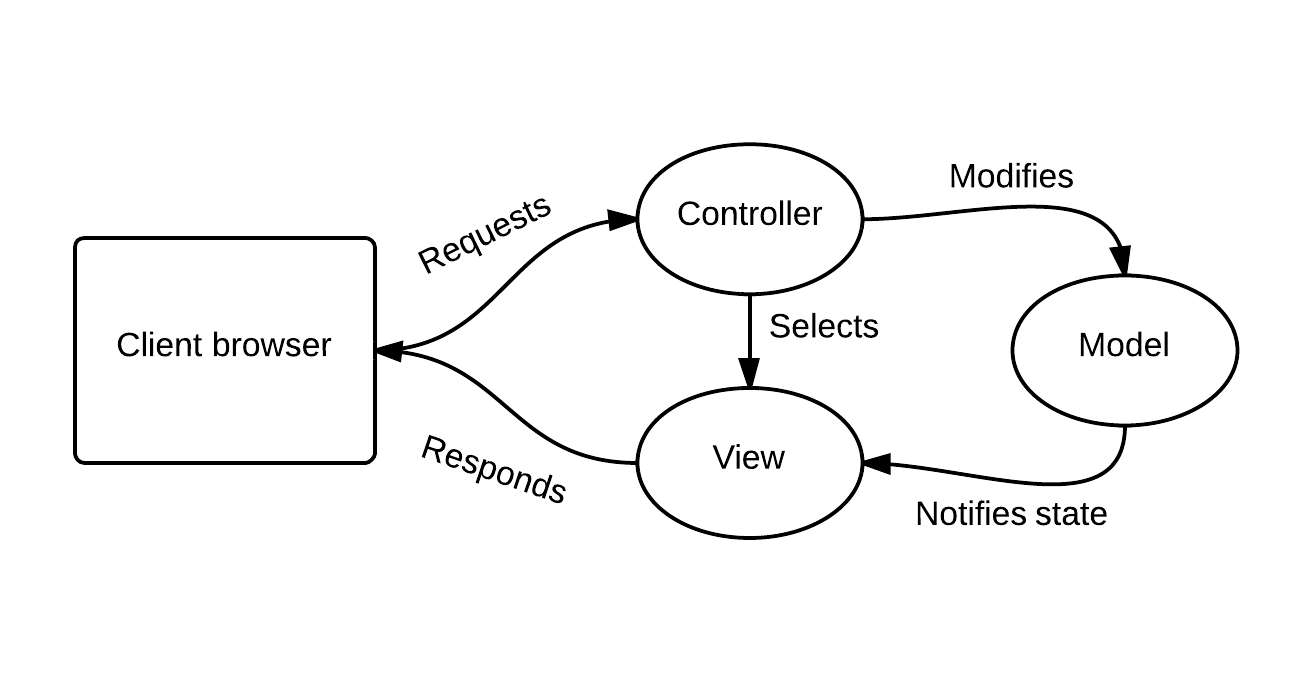
\includegraphics[width=\textwidth]{img/mvc.png}
\caption{Overview of the MVC workflow.}
\label{fig:mvc}
\end{figure}

\textbf{Model:} contains the logic, which is usually designed in such a way, that it can be reused and shared with other applications.
The model ignores how user requests are issued and how data is represented to the user.\newline

\textbf{View:} handles the representation of data for the end users.
It is possible for an application to have multiple different views for use in various situations.
The view ignores the form of user requests and the source of the data.\\

\textbf{Controller:} manages user interactions and instantiates the model and view based on performed actions, user rights and the like.
The controller ignores the logic of the model and the presentation of the view.

\todo{From Martin: You have described MVC nicely but what is the relation to your project? Why not use it in our project? (if you have not implemented it.)}